\chapter{Semafori}

\section{Introduzione}

\dfn{Semaforo}{Un \newfancyglitter{semaforo} è un tipo di dato astratto\footnote{Opaco, non si sa com'è implementato.}, che assume valori interi ì, $\geq$ 0, su cui si eseguono solo due primitive atomiche: P e V (wait, signal).}

\nt{Una variabile di tipo \fancyglitter{semaphore} è condivisibile da due o più processi.}

\clm{}{}{ 
  \begin{itemize}
    \item Strumento linguistico di "basso livello" per \fancyglitter{problemi di sincronizzazione}. 
    \item Normalmente realizzato a \fancyglitter{livello macchina} per realizzare strumenti di sincronizzazione di "più alto livello". 
    \item Disponibile in librerie standard per la realizzazione di programmi concorrenti con linguaggi sequenziali. 
  \end{itemize}
}

\cor{P}{
La P prova ad accedere al semaforo. Quando accede decrementa il contatore di 1. 
} 

\begin{center}
   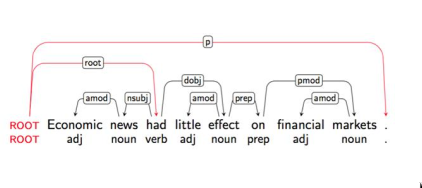
\includegraphics[scale=0.4]{03-Semafori/P.png}
\end{center}

\cor{V}{
Incremena di 1 il contatore.
}

\begin{center}
   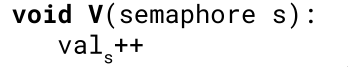
\includegraphics[scale=0.4]{03-Semafori/V.png}
\end{center}

\paragraph{Un semaforo è:}

\begin{itemize}
  \item \fancyglitter{Generalev(o contatore):} se il suo valore può assumere qualsiasi valore intero non negativo. 
  \item \fancyglitter{Binario:} se può assumere solo i valori 0 e 1 (la V aumenta solo se il valore corrente è 0).
\end{itemize}

\subsubsection{Implementazione dei Semafori}

La definizione di Dijkstra, essendo astratta, non tiene conto degli aspetti implementativi. Per quanto riguarda l'operazione P sono disponibili varie soluzioni:

\begin{itemize}
  \item \fancyglitter{Busy Waiting:} attesa attiva, \textit{spinlock}. 
  \item \fancyglitter{Insieme di processi bloccati}. 
  \item \fancyglitter{Coda FIFO di processi bloccati}.
\end{itemize}

\nt{In questo corso non si faranno assunzioni sul tipo di implementazione, ma solamente sulla gestione fair dei processi bloccati.}

\subsection{Invarianti Semaforici}

\dfn{Invariante Semaforico}{ 
  \begin{itemize}
  \item $I_{sem}$: valore intero $\geq$ 0 con cui il semaforo \newfancyglitter{sem} viene inizializzato.
  \item $NV_{sem}$: numero di volte che l'operazione V(sem) è stata \textit{eseguita} fino allo stato s. 
  \item $NP_{sem}$: numero di volte che l'operazione P(sem) è stata \textit{completata} fino allo stato s. 

\end{itemize}

$$val_{sem}(s) = I_{sem} + NV_{sem}(s) - NP_{sem}(s), \text{ con } val_{sem} \geq 0$$

In ogni stato vale: 

$$NP_{sem} \leq I_{sem} + NV_{sem}$$

}

\subsubsection{Il Problema della Mutua Esclusione}

Il problema della mutua esclusione tra un insieme di processi si può risolvere con l'utilizzo di un semaforo binario chiamato \fancyglitter{mutex}. 

\dfn{Mutex}{ 
Il mutex è un semaforo binario inizializzato a 1 con semantica: 
\begin{itemize}
  \item val(mutex) = 1, la sezione critica è libera. 
  \item val(mutex) = 0, la sezione critica è stata acquisita da un processi.
\end{itemize}

Il \newfancyglitter{prologo} per l'accesso alla CS è costituito dall'operazione P(mutex) e l'\newfancyglitter{epilogo} dall'operazione V(mutex).

}


\begin{center}
   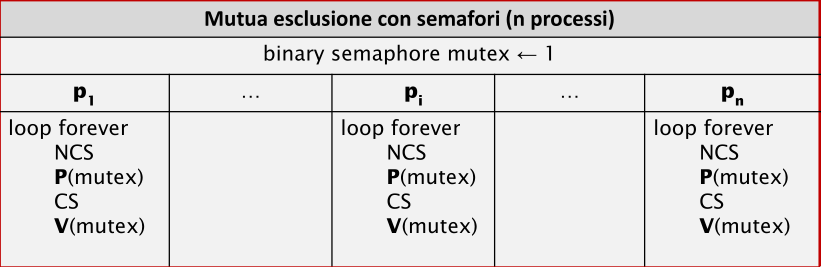
\includegraphics[scale=0.4]{03-Semafori/ME.png}
\end{center}

\paragraph{Una buona soluzione ha:}

\begin{itemize}
  \item \fancyglitter{Mutua Esclusione}. 
  \item \fancyglitter{Assenza di Deadlock}. 
  \item \fancyglitter{Assenza di Starvation}. 
\end{itemize}

\nt{L'assenza di starvation dipende strettamente dall'implementazione dei semafori, quindi si può assumere (ipotesi strong).}

\begin{center}
   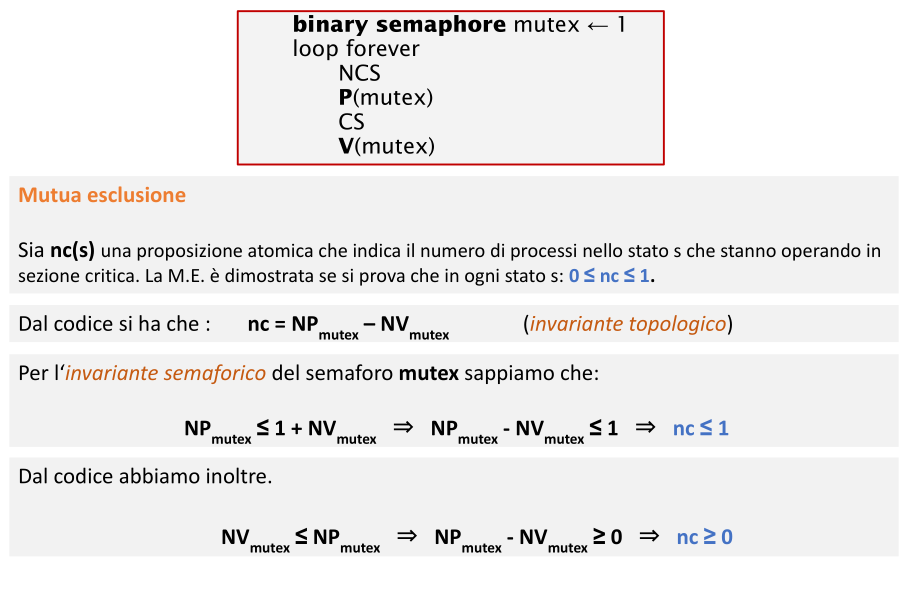
\includegraphics[scale=0.4]{03-Semafori/MEP.png}
\end{center}



\begin{center}
   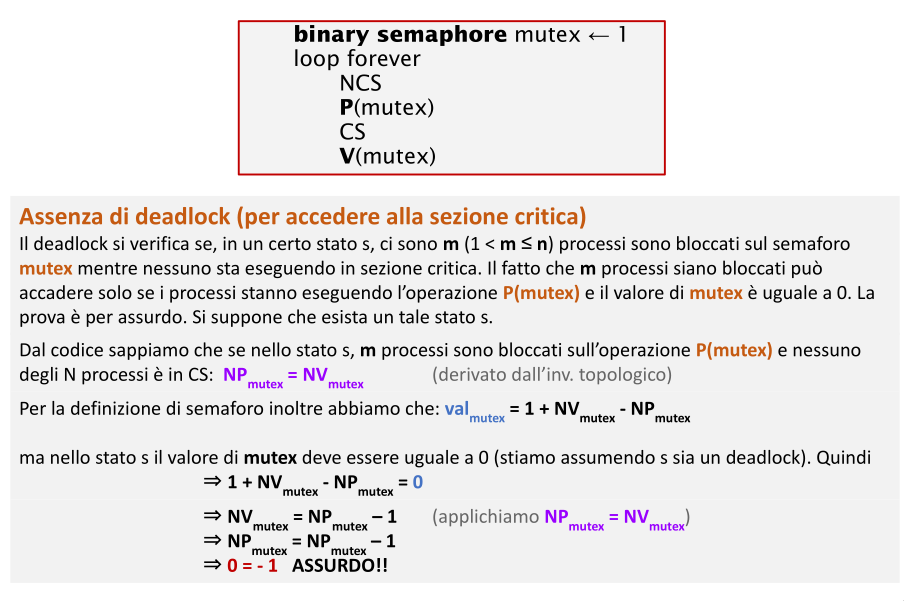
\includegraphics[scale=0.4]{03-Semafori/ADP.png}
\end{center}

\subsection{Semafori per lo Scambio di Segnali Temporali} 

Un uso frequente dei semafori è quello di imporre un ordine di esecuzione tra le operazioni dei processi concorrenti.

\begin{center}
   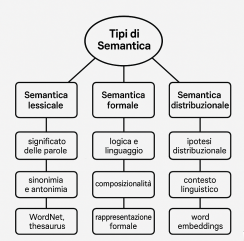
\includegraphics[scale=0.4]{03-Semafori/sem.png}
\end{center}


\dfn{Barriera Sincrona}{ 
La \newfancyglitter{barriera sincrona} (o Rendezvous sincrono) tra due processi: 

\begin{itemize}
  \item Due processi P e Q eseguono ciascuno due operazioni consecutive. Pa e Pb il primo, Qa e Qb il secondo. 
  \item \newfancyglitter{Vincolo di barriera:} l'esecuzione di Pb da parte di P e quella di qb da parte di Q possono iniziare solo dopo che entrambi i processi hanno completato la loro prima operazione.
\end{itemize}
}

\begin{center}
   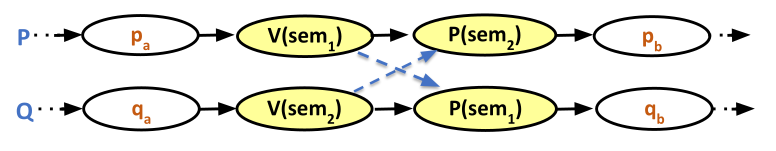
\includegraphics[scale=0.4]{03-Semafori/BS.png}
\end{center}

\subsection{Prove di Correttezza}

\subsubsection{Produttore-Consumatore con un Buffer Infinito}

\begin{itemize}
  \item Due processi, produttore e consumatore, si scambiano dati di tipo \fancyglitter{type} utilizzando un buffer condiviso infinito. 
  \item Il consumatore non deve cercare di prelevare un dato dal buffer quando questo è vuoto. Se il consumatore trova il buffer vuoto deve attendere. 
  \item Si suppone che \fancyglitter{take} e \fancyglitter{append} siano atomiche.
\end{itemize}

\begin{center}
   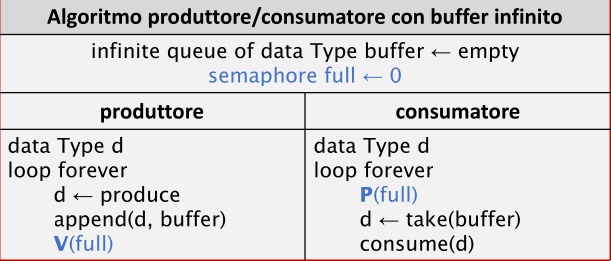
\includegraphics[scale=0.4]{03-Semafori/ProdCons.png}
\end{center}

\subsubsection{Produttore-Consumatore con un Buffer Limitato}

\begin{itemize}
  \item Due processi, produttore e consumatore, si scambiano dati di tipo \fancyglitter{type} utilizzando un buffer condiviso in grado di contenere max dati. 
  \item Il consumatore non deve cercare di prelevare un dato dal buffer quando questo è vuoto. Se il consumatore trova il buffer vuoto deve attendere. 
  \item Il produttore non deve cercare di inserire un dato nel buffer quando questo è pieno.
  \item Si suppone che \fancyglitter{take} e \fancyglitter{append} siano atomiche.
\end{itemize}

\begin{center}
   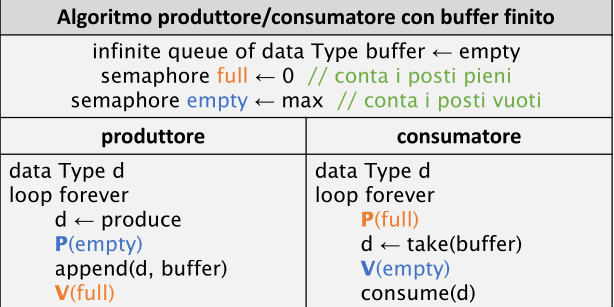
\includegraphics[scale=0.4]{03-Semafori/ProdCons2.png}
\end{center}

\subsubsection{Produttore-Consumatore con un Buffer Circolarede}

\begin{itemize}
  \item
\end{itemize}

\begin{center}
   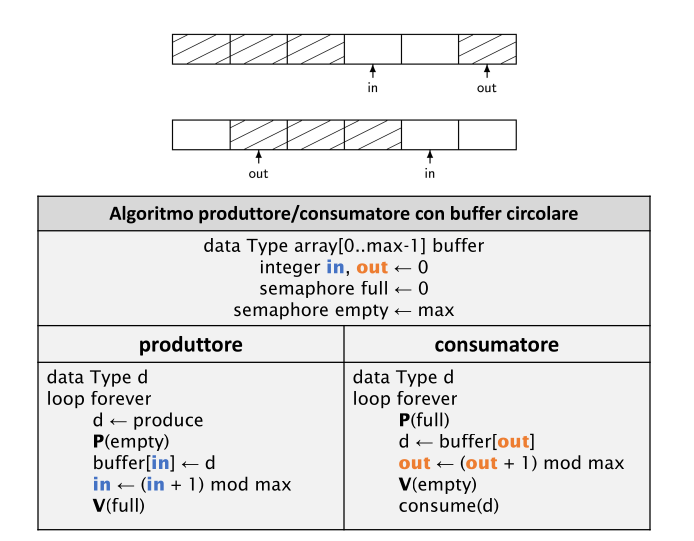
\includegraphics[scale=0.4]{03-Semafori/ProdConsC.png}
\end{center}







